\chapter{Programming Principles}
\section{SOLID}
\paragraph{Single responsibility principle}
Die meisten Klassen in der Anwendung erfüllen das Prinzip und haben nur eine Zuständigkeit. Ein gutes Beispiel ist der \href{https://github.com/EinToni/Wortfinder/blob/main/Wortfinder/GameTimer.cs}{\textit{GameTimer}} welcher nur einen Timer starten sowie stoppen kann und bei jedem Tick eine Callback Funktion aufruft. Ein Beispiel für eine Klasse welches es nicht erfüllt hat, ist der \href{https://github.com/EinToni/Wortfinder/blob/main/Wortfinder/MainWindowController.cs}{\textit{MainWindowController}}. Dieser war zum einen der Adapter zwischen dem \href{https://github.com/EinToni/Wortfinder/blob/main/Wortfinder/MainWindow.xaml.cs}{\textit{MainWindow}} und dem \href{https://github.com/EinToni/Wortfinder/blob/main/Wortfinder/GameManager.cs}{\textit{GameManager}}, hat aber auch das Verbinden von Buchstaben in der GUI kontrolliert. Die Funktionalitäten zum Verbinden von Buchstaben wurde daher in eine neue Klasse \href{https://github.com/EinToni/Wortfinder/blob/main/Wortfinder/WordBuilder.cs}{\textit{WordBuilder}} ausgelagert, Commit \href{https://github.com/EinToni/Wortfinder/commit/817e4b1b6be02defe58792a4afb709c7a147ced5}{817e4b1b6be02defe58792a4afb709c7a147ced5} und der darauf folgende. 


\paragraph{Open/Closed principle}
Eine auffällige Verbesserungsmöglichkeit wurde im \href{https://github.com/EinToni/Wortfinder/blob/main/Wortfinder/GameScoreCalculator.cs}{\textit{GameScoreCalculator}} gefunden, welcher immer wieder modifiziert wurde um die Punktzahl anders zu berechnen. Die Berechnung wurde nun Erweiterbar ausgelagert. Dafür wurde eine Liste im \href{https://github.com/EinToni/Wortfinder/blob/main/Wortfinder/GameScoreCalculator.cs}{\textit{GameScoreCalculator}} erstellt welche Klassen eines \href{https://github.com/EinToni/Wortfinder/blob/main/Wortfinder/Interfaces/IPointFactor.cs}{\textit{IPointFactor}} Interfaces beinhaltet. Über diese wird beim Berechnen der Punkte Iteriert und jede Klasse berechnet dann einen Teilbetrag der Punktzahl, bezogen auf einen bestimmten Faktor. Siehe Commit \href{https://github.com/EinToni/Wortfinder/commit/6a4834cfc653a63ed3efc8745bccbe603250da74}{6a4834cfc653a63ed3efc8745bccbe603250da74} sowie die folgende Abbildung:

\begin{figure}[!htb]
\centering
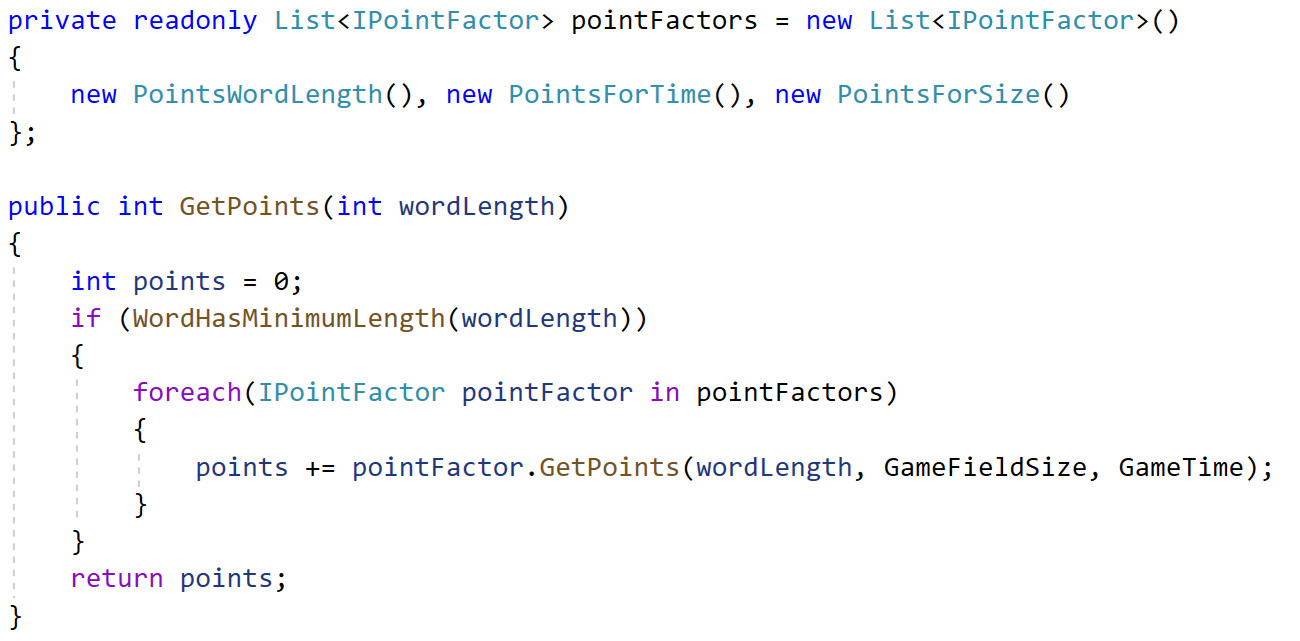
\includegraphics[width=0.7\textwidth]{Bilder/openClosedExample.PNG}
\caption{\label{Abb:openClosedExample}Erweiterbare Berechnung der Punktzahl für ein Wort}
\end{figure}

\paragraph{Liskov substitution principle}
Das Liskov substitution principle ist erfüllt, da Vererbung nur bei Interfaces verwendet wurde.

\paragraph{Interface Segregation principle}

\paragraph{Dependency inversion principle}
Dependency inversion wurde im Rahmen der Implementierung der Clean Architecture angewendet. Dabei wurden die Abhängigkeiten durch die Einführung von Interfaces bei den betroffenen Klassen an den Grenzen der einzelnen Schichten umgekehrt, wie in Kapitel~\ref{cleanArchitecture} Clean Architecture in Abbildung~\ref{Abb:DependencyInversion} gezeigt.

\section{GRASP}
\paragraph{Grundkonzept} 
%% Hohe Kopplung
Der Code hat stellenweise eine recht hohe Kopplung, da oft Funktionen innerhalb der selben Klasse statisch aufgerufen werden. Ein Beispiel dafür ist die \href{https://github.com/EinToni/Wortfinder/blob/main/Wortfinder/WordGenerator.cs}{\textit{WordGenerator}} Klasse. Diese besteht aus 6 Funktionen, von welchen nur die erste von einer anderen Klasse aufgerufen wird. Alle anderen werden als statische Methodenaufrufe innerhalb der Klasse selbst aufgerufen. Diese Aufrufe stehen fest im Code und sind daher nicht austauschbar wodurch sich eine starke Koppelung ergibt.

%% Niedrige Kopplung
Im Vergleich dazu ist ein Beispiel für lose Kopplung die \href{https://github.com/EinToni/Wortfinder/blob/main/Wortfinder/GameManager.cs}{\textit{GameManager}} Klasse. Diese macht primär Aufrufe an Interfaces welche austauschbarer sind und ist daher recht lose gekoppelt.

%% Hohe Kohäsion
Eine hohe Kohäsion findet sich beispielsweise in der \href{https://github.com/EinToni/Wortfinder/blob/main/Wortfinder/Coordinate.cs}{\textit{Coordinate}} Klasse wieder. Diese hält zwei Ganzzahlen, welche für den X und Y Wert der Koordinate stehen und stellt Methoden zur Verfügung, welche die Zahlen verwenden um sie mit einer anderen \href{https://github.com/EinToni/Wortfinder/blob/main/Wortfinder/Coordinate.cs}{\textit{Coordinate}} Instanz zu vergleichen oder umzurechnen. Semantisch sind alle Methoden und Attribute somit sehr nah.


\paragraph{Code-Strukturierung}
Es wird viel Indirektion verwendet. Ein gutes Beispiel dafür ist der \href{https://github.com/EinToni/Wortfinder/blob/main/Wortfinder/GameManager.cs}{\textit{GameManager}}, welcher im Grunde alle Aufrufe an verschiedene andere Klassen bzw. Interfaces weiterleitet. Somit delegiert dieser andere Klassen und lässt diese für sich Arbeiten.


\paragraph{Architektur}
\glqq Pure fabrication\grqq{} findet sich beispielsweise in der \href{https://github.com/EinToni/Wortfinder/blob/main/Wortfinder/EnDecrypter.cs}{\textit{EnDecoder}} Klasse wieder. Diese ist unabhängig von jeglicher Anwendungslogik und ver- bzw. entschlüsselt einen beliebigen Stream mit einem beliebigen key in ein beliebiges Verzeichnis. Somit lässt sich diese allgemein zum ver- und entschlüsseln von Streams verwenden und hat keinerlei Bezug zur Problemdomäne.


\paragraph{Entwurfsmuster}
Die GUI Elemente (außer das UserControll Element \href{https://github.com/EinToni/Wortfinder/blob/main/Wortfinder/WordDisplay.xaml.cs}{\textit{WordDisplay}}) kommuniziert immer nur mit einen Controller. Ein Beispiel ist der \href{https://github.com/EinToni/Wortfinder/blob/main/Wortfinder/MainWindowController.cs}{\textit{MainWindowController}}. Dieser Leitet die Aufrufe weiter und bestimmt wer den Aufruf weiter verarbeitet, der \textit{WordBuilder} oder \textit{GameManager}. Dabei wandelt er teilweise auch Datentypen um.


\section{DRY}
Das \glqq don't repeat yourself\grqq{} Prinzip wurde im Produktivcode meistens eingehalten, da versucht wurde die mehrfach verwendeten Informationen als Variablen in Klassen zu speichern und wiederzuverwenden. Somit sind die Informationen nur an einem Ort gespeichert. Ein Beispiel für die Einhaltung ist die \href{https://github.com/EinToni/Wortfinder/blob/main/Wortfinder/GameLibrary.cs}{\textit{GameLibrary}} Klasse, welche überprüft das eine gewisse Anzahl an generierten Spielen existiert. Diese Anzahl ist als Variable in der Klasse gespeichert und wird mehrfach verwendet. Somit müsste, zum ändern der Anzahl der zu generierenden Spiele, nur diese eine Variable geändert werden.


Innerhalb von Tests wurde das Prinzip allerdings häufig nicht eingehalten. Weil die Tests oft schnell geschrieben wurden, wurden oftmals keine extra Variablen angelegt, sondern die Informationen mehrfach direkt verwendet. Die Anpassungen von einigen Tests sind in Commit \href{https://github.com/EinToni/Wortfinder/commit/31e056a85512623173a8e4efa2faa828b2f66466}{31e056a85512623173a8e4efa2faa828b2f66466}.
\endinput